
\noindent\begin{minipage}{\textwidth}
    \begin{table}[H]
        \centering
        \caption{Hiperparâmetros e Resultados do Melhor Modelo - convnext\_v11\_AM\_opt\_aug}
        \vspace{0.2cm}
        \resizebox{\textwidth}{!}{%
            \begin{tabular}{ll | lrrr}
                \hline
                \multicolumn{2}{c|}{\textbf{Hiperparâmetros}} & \multicolumn{4}{c}{\textbf{Métricas por Classe}} \\ \hline
                \textbf{Parâmetro} & \textbf{Valor} & \textbf{Classe} & \textbf{Precisão} & \textbf{Recall} & \textbf{F1-Score} \\ \hline
    Agendador (\$T\_0\$) & 7 & 31.2 & 0.7167 & 0.1903 & 0.3007 \\ 
Agendador de LR & CosineAnnealingWarmRestarts & 31.3 & 0.2346 & 0.1881 & 0.2088 \\ 
Architecture & convnext\_tiny & 31.4 & 0.2018 & 0.4286 & 0.2744 \\ 
Batch Size & 32 & 32.3 & 0.3224 & 0.3010 & 0.3113 \\ 
Data Augmentation & False & 32.4 & 0.3158 & 0.1034 & 0.1558 \\ 
Decaimento de Peso (WD) & 0.0351 & 33.3 & 0.1849 & 0.2798 & 0.2227 \\ 
Dropout & 0.3486 & 41.4 & 0.2000 & 0.0682 & 0.1017 \\ 
Função de Perda & CrossEntropyLoss & 41.5 & 0.6250 & 0.1282 & 0.2128 \\ 
Hidden Units & 512 & 42.4 & 0.1972 & 0.2059 & 0.2014 \\ 
Label Smoothing & 0.1663 & 44.4 & 0.2222 & 0.0690 & 0.1053 \\ 
\cline{3-6} 
Otimizador & AdamW & \textbf{Média (Macro)} & 0.2358 & 0.2278 & 0.2181 \\ 
Taxa de Aprendizado (LR) & 1.14e-04 & \textbf{MCC} & \multicolumn{3}{c}{0.1539} \\ 
Unfreeze Layers & 5 &  & & &  \\ 
            \hline
            \end{tabular}%
        }
    \end{table}

    \begin{figure}[H]
        \centering
        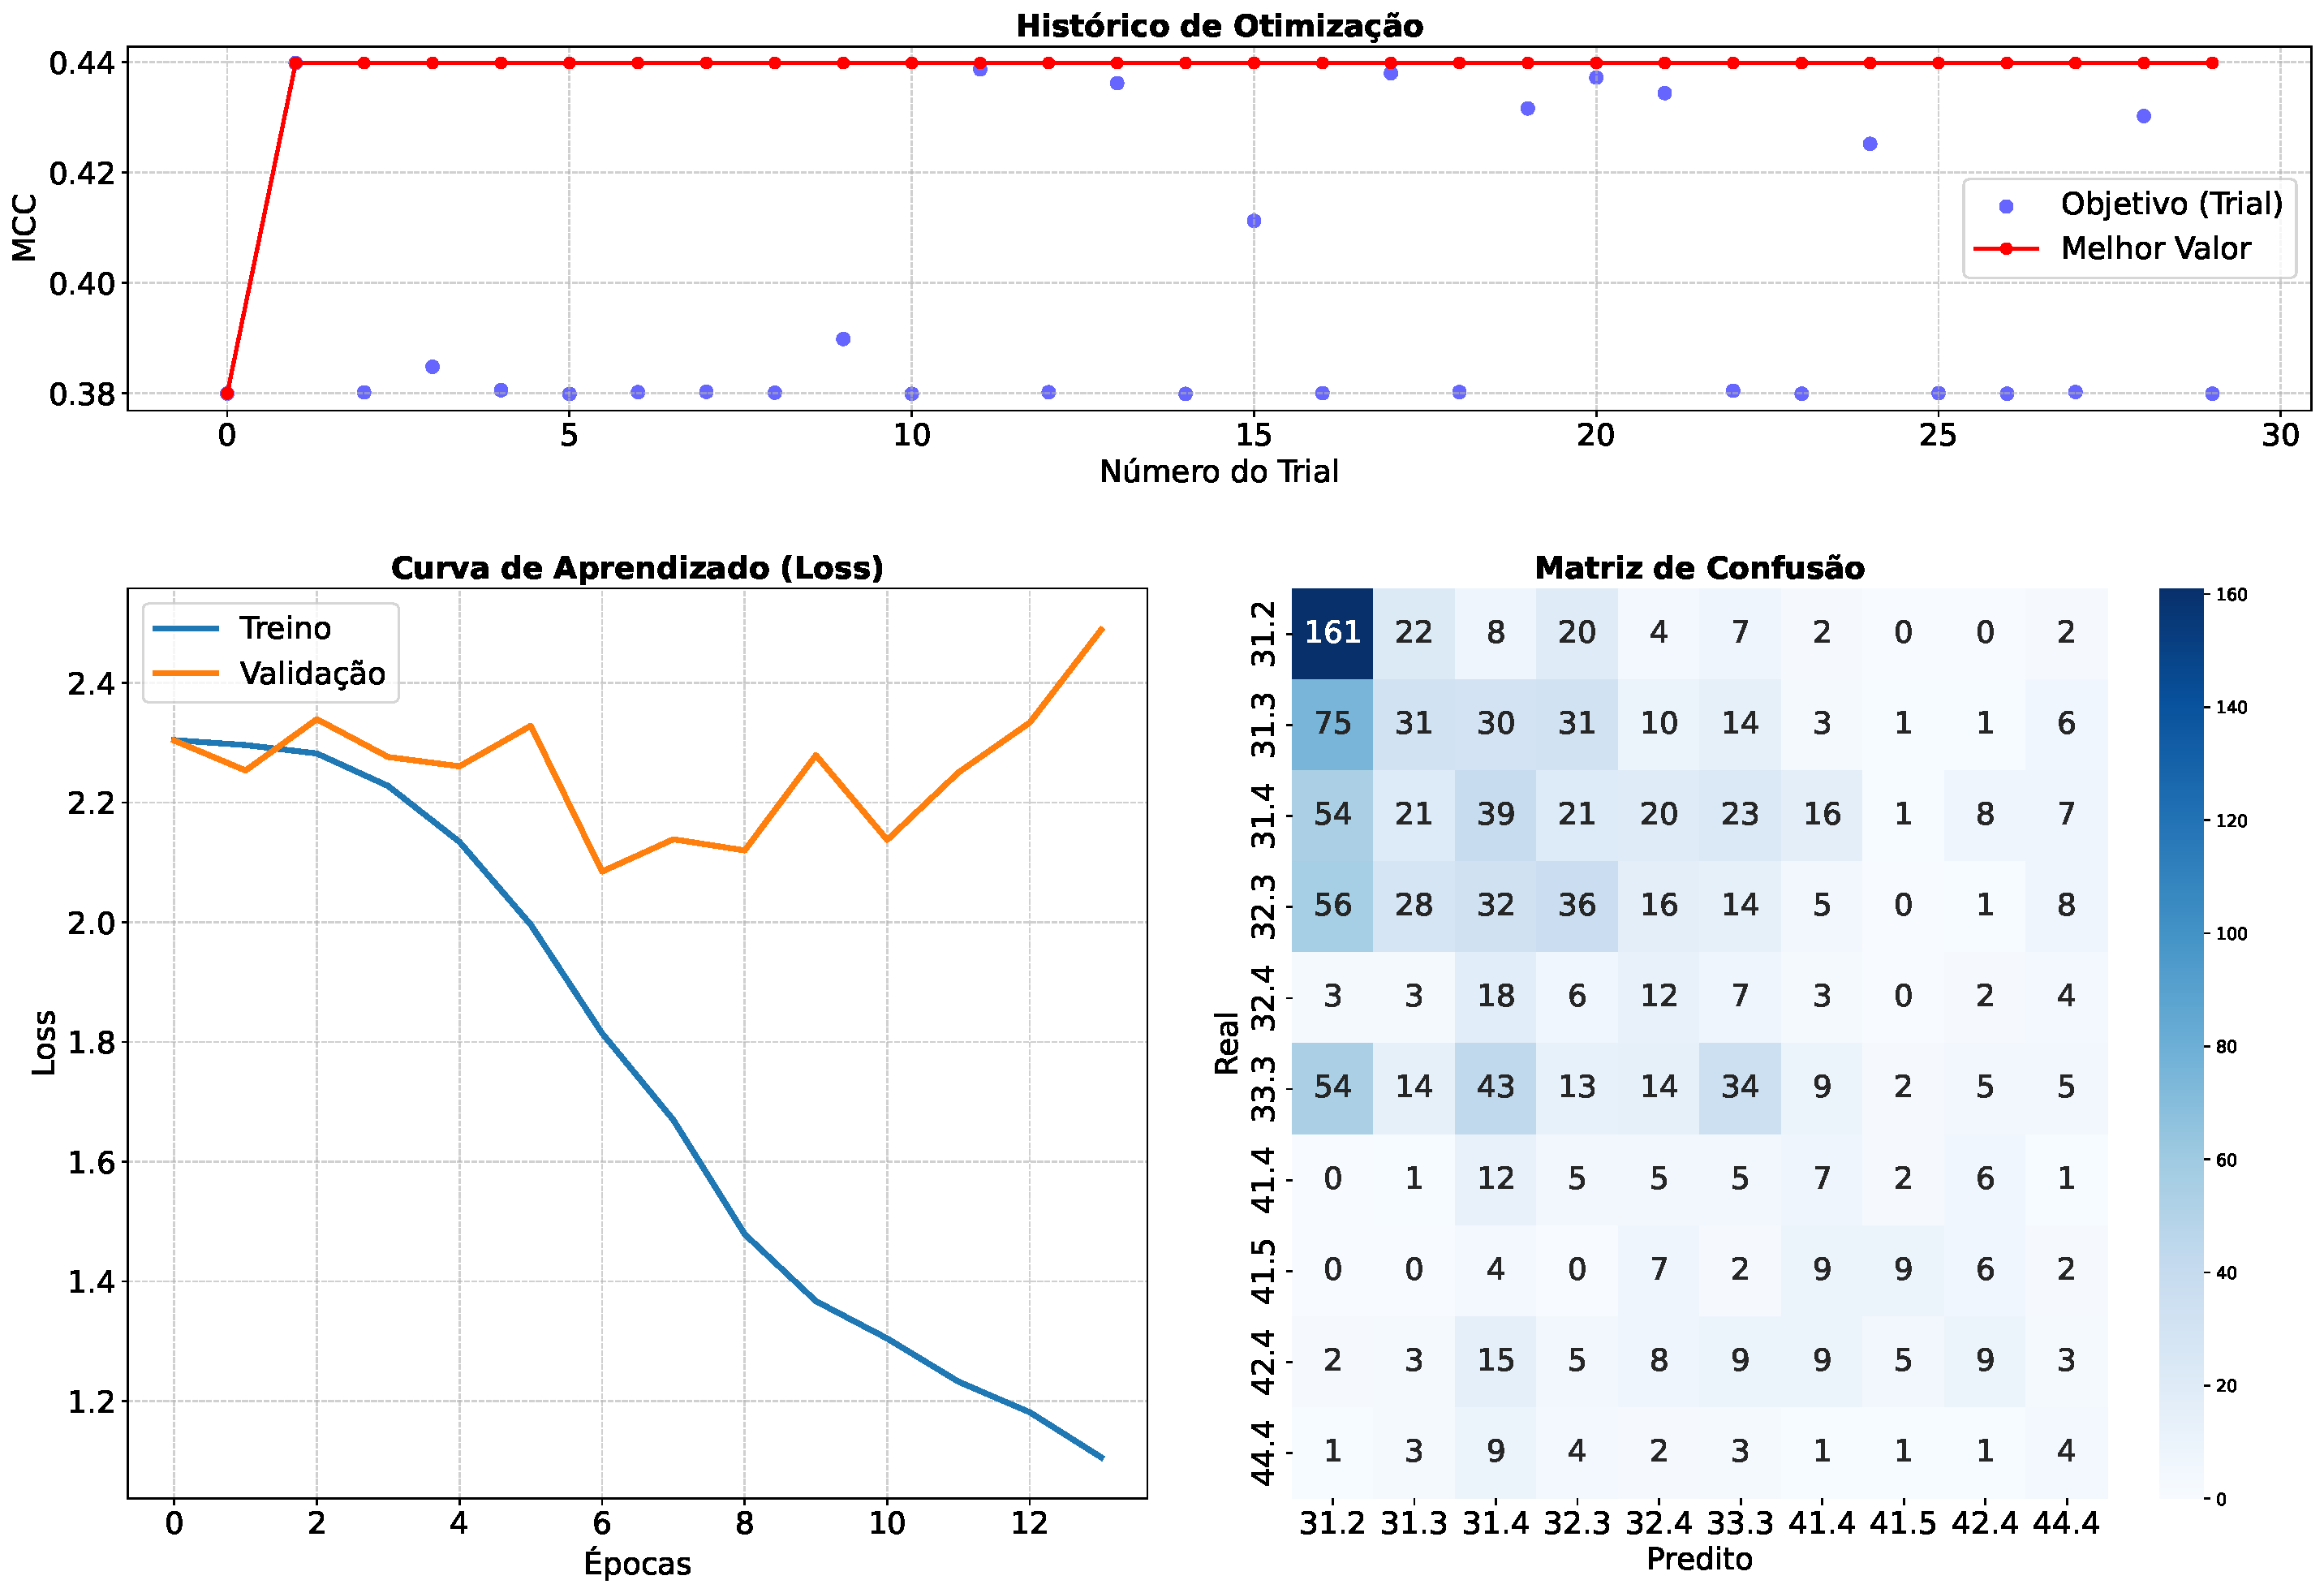
\includegraphics[width=0.85\textwidth]{tex/appendix/experiments/convnext_v11_AM_opt_aug/dashboard_consolidado.pdf}
        \caption{Histórico de Otimização, Curvas de Aprendizado e Matriz de Confusão - convnext\_v11\_AM\_opt\_aug}
    \end{figure}
\end{minipage}
\clearpage
